\subsubsection{Use Cases}
In the following section we will present the use case diagram and the use cases made to uncover the functional requirements for the system.

\subsubsubsection{Use case diagram}
We have produced a use case diagram, see \fref{useCaseImg}, which outlines the boundaries of the system, and how the different actors (user types) can interact with the server. 
\begin{figure}[h]
\centering
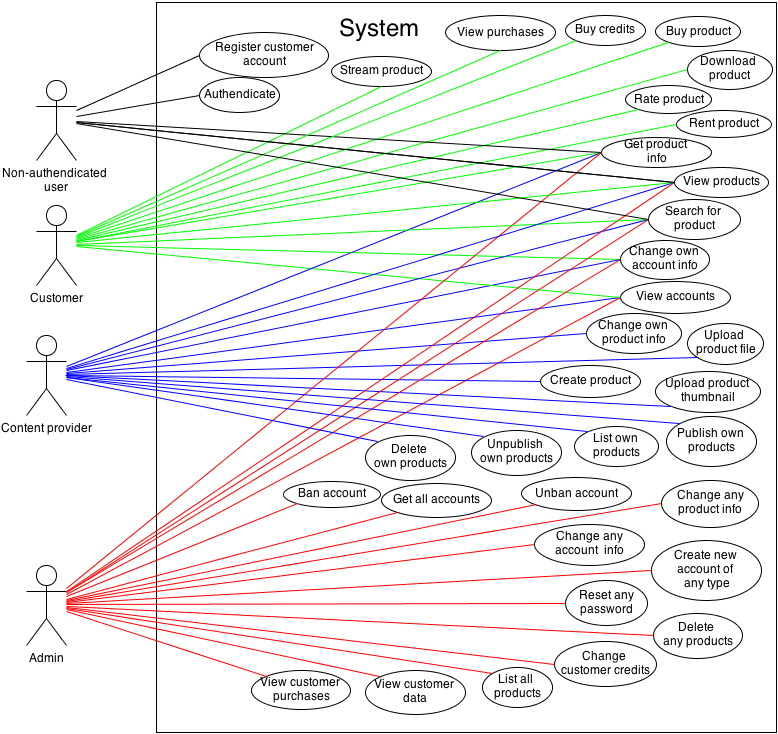
\includegraphics[scale=0.5]{illustrations/UseCaseDiagram.png}
\caption{Use case diagram for our web service}
\label{useCaseImg}
\end{figure}

\subsubsubsection{Use cases}
In the following section example use cases for our system is listed. Every use case has a short description of the scenario it is representing, its pre- or postconditions if any, and then its basic flow and success scenario.\\
Only two use cases are listed here. For a complete list of our use cases, see \apref{Apendix_usecases}

\vspace{3mm}
\textbf{Success scenario: Buy product} \\
Spiderman wants to buy the movie 'The Dark Knight'. 
\begin{tabbing}
\hspace{5mm}\=\hspace{26mm}\=\kill
\>Primary Actor:\> Customer\\
\>Precondition:\> The actor is logged in and it is possible to buy the\\ \hspace{85px} product.\\
\>Postcondition:\> The actor has bought the product and the credits is\\ \hspace{85px} withdrawn from the actors account.
\end{tabbing}
\begin{enumerate} \setlength{\itemsep}{-1mm}
	\item Spiderman navigates to the movie.
	\item He clicks the 'buy product' link.
\end{enumerate}

\vspace{3mm}
\textbf{Success scenario: Rate product} \\
Spiderman wants to rate the movie 'The Dark Knight'. 
\begin{tabbing}
\hspace{5mm}\=\hspace{26mm}\=\kill
\>Primary Actor:\> Customer\\
\>Precondition:\> The product is published.\\
\>Postcondition:\> The average rating of the product is changed accordingly\\ \hspace{85px} to the new rating.
\end{tabbing}
\begin{enumerate} \setlength{\itemsep}{-1mm}
	\item Spiderman navigates to the movie.
	\item He rates the product on a scale from -5 to 5.
\end{enumerate}